\section{Triplets}
%
% - Purpose & Problem description:
%     These first two parts give reader short details about the test case,
%     the physical phenomena involved and specify how the numerical solution will be validated
%
\subsection{Purpose}
%
This test case has been created to test the extend the covering by using option of triad interactions that were not used in other cases. 

%
\subsection{Description of the problem}
We simulate non linear transfers between triads. In the first case we use Lumped Triad Approximation model (LTA) and in the second case we use the SPB model 
\begin{figure} [!h]
\centering
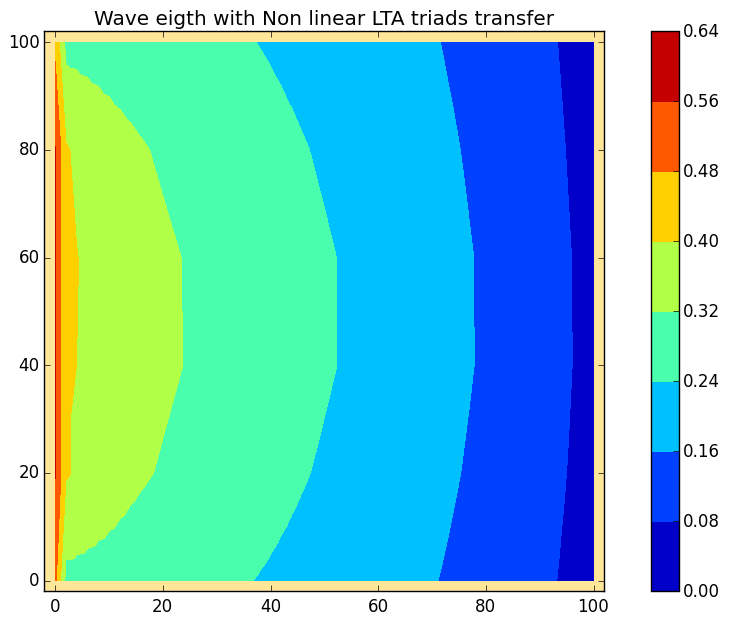
\includegraphics[scale = 0.65]{../results.png}
 \caption{Wave height for Lumped Triad Approximation model}
\label{figrestripl}
\end{figure}
\begin{figure} [!h]
\centering
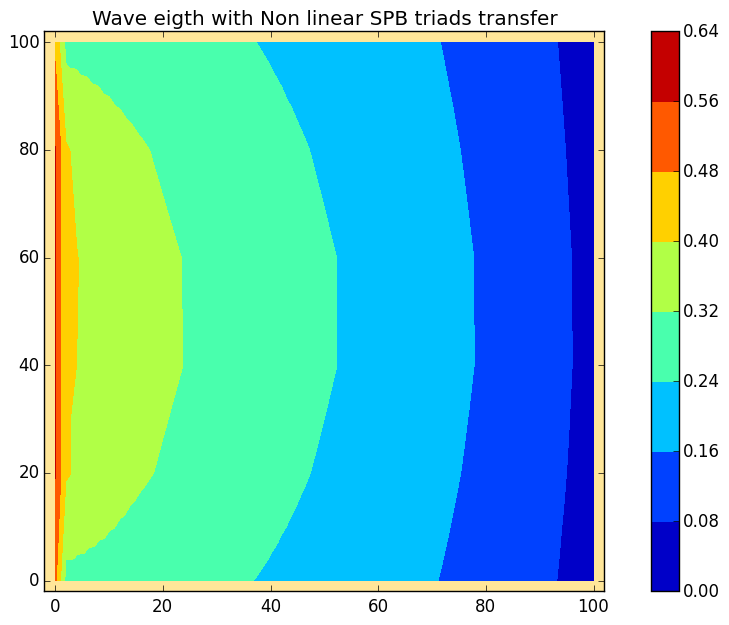
\includegraphics[scale = 0.65]{../results2.png}
 \caption{Wave height for SPB model}
\label{figrestripl2}
\end{figure}
